\chapter{椭圆型方程的有限差分法}
\section{2.1}
椭圆方程就是最高阶是两阶
\begin{definition}[区间剖分与步长]
设区间为 \([a,b]\)。将 \([a,b]\) 分成 \(N\) 等分，分点取为
\[
x_i=a+ih,\qquad i=0,1,\dots,N,
\]
其中
\[
h=\frac{b-a}{N}.
\]
由这些分点得到的点列 \(\{x_i\}_{i=0}^N\) 称为区间 \([a,b]\) 的一个剖分，点 \(x_i\) 称为节点，常数 \(h\) 称为步长。
\end{definition}
所以“差分法”本质上就是：
把连续的导数，换成离散点上的差商。
\begin{enumerate}
    \item 原问题：先有边值问题 \(-u''+qu=f,\ u(a)=\alpha,\ u(b)=\beta\)。
    \item 剖分区间：把 \([a,b]\) 切成很多小段，得到节点 \(x_i\)。
    \item 导数离散化：用中心差分 \(u''(x_i)\approx \dfrac{u_{i+1}-2u_i+u_{i-1}}{h^2}\)。
    \item 代回方程：得到离散方程 \(-\dfrac{u_{i+1}-2u_i+u_{i-1}}{h^2}+q_i u_i=f_i\)。
    \item 加边界条件：\(u_0=\alpha,\ u_N=\beta\)。
    \item 结果：连续微分方程变成一个线性方程组，解这个方程组，就得到各节点上的近似值。
\end{enumerate}
\begin{example}
用差分法求边值问题 \(-u''=1,\ 0<x<1,\ u(0)=0,\ u(1)=0\) 的近似解。

将区间 \([0,1]\) 分成 \(N=2\) 等分，则步长 \(h=\frac12\)，节点为 \(x_0=0,\ x_1=\frac12,\ x_2=1\)。在内部节点 \(x_1\) 处，用中心差分近似二阶导数：
\[
u''(x_1)\approx \frac{u_2-2u_1+u_0}{h^2}.
\]
原方程为 \(-u''=1\)，代入得
\[
-\frac{u_2-2u_1+u_0}{h^2}=1.
\]
再代入 \(h=\frac12,\ u_0=0,\ u_2=0\)，得
\[
-\frac{0-2u_1+0}{(1/2)^2}=1,
\]
即 \(8u_1=1\)，所以
\[
u_1=\frac18.
\]

因此在节点处的近似解为 \(u_0=0,\ u_1=\frac18,\ u_2=0\)。
\end{example}
\begin{dxtips}
    也就是为了确定让两头等于固定的值，二阶导也等于固定的值，通过差分法把二阶导表示出来。然后差分也能用到首项和末项的值，所以这个等式成立以后只有一个未知数就是中间那个点点值
\end{dxtips}
\begin{example}
用差分法将边值问题 \(-u''=1,\ 0<x<1,\ u(0)=0,\ u(1)=0\) 化为线性方程组。

将区间 \([0,1]\) 分成 \(N=4\) 等分，则步长 \(h=\frac14\)，节点为 \(x_0=0,\ x_1=\frac14,\ x_2=\frac12,\ x_3=\frac34,\ x_4=1\)。边界条件给出 \(u_0=0,\ u_4=0\)。对内部节点 \(x_1,x_2,x_3\)，由中心差分近似 \(u''(x_i)\approx \dfrac{u_{i+1}-2u_i+u_{i-1}}{h^2}\)，代入方程 \(-u''=1\)，得
\[
-\frac{u_{i+1}-2u_i+u_{i-1}}{h^2}=1,\qquad i=1,2,3.
\]
再代入 \(h=\frac14\)，可得
\[
\begin{cases}
-\,u_2+2u_1-u_0=\dfrac{1}{16},\\\\
-\,u_3+2u_2-u_1=\dfrac{1}{16},\\\\
-\,u_4+2u_3-u_2=\dfrac{1}{16}
\end{cases}
\quad \Longrightarrow \quad
\begin{cases}
2u_1-u_2=\dfrac{1}{16},\\
-u_1+2u_2-u_3=\dfrac{1}{16},\\
-u_2+2u_3=\dfrac{1}{16}
\end{cases}
\]
这就是对应的线性方程组。
\end{example}
\begin{enumerate}
    \item 范数用来衡量“一个网格函数有多大”以及“两个近似解差多少”。
    \item 分析误差：想说数值解和真解接近，必须先规定“接近”按什么量来量。
    \item 讨论收敛：当 \(h\to 0\) 时，\(\|u-u_h\|\to 0\) 才叫收敛。
    \item 讨论稳定性：右端稍微变一点，解会不会暴涨，要靠范数控制。
    \item 所以范数不一定直接拿来“算出解”，但它是分析“解得好不好、稳不稳、误差多大”的工具。
\end{enumerate}
\begin{definition}[相容性条件]
设 \(M\) 是某一充分光滑函数类，\(R_h(u)\) 是由截断误差定义的网格函数。若对任意 \(u\in M\)，恒有
\[
\lim_{h\to 0}\|R_h(u)\|=0,
\]
则称该差分算子逼近于原微分算子，或称该差分格式满足\textbf{相容性条件}。
\end{definition}

\begin{note}。步长足够小时，差分算子对微分算子的近似越来越好；若再有稳定性，数值解才会收敛。
\end{note}
\begin{definition}[收敛性]
称差分解 \(u_h\) 收敛到边值问题的解 \(u\)，如果当 \(h\) 充分小时，差分方程的解 \(u_h\) 存在，且按某一范数有
\[
\lim_{h\to 0}\|u_h-u\|=0,
\]
这里把 \(u\) 看成 \(I_h\) 上的网格函数。
\end{definition}

\begin{note}
根据差分方程格式，有
\[
L_hu(x_i)=f_i+R_i(u),
\qquad
L_hu_i=f_i.
\]
引进误差
\[
e_i=u(x_i)-u_i,
\]
两式相减得
\[
\begin{cases}
L_he_i=R_i(u), & i=1,2,\cdots,N-1,\\
e_0=e_N=0.
\end{cases}
\]
于是，收敛性和收敛速度的估计问题，就归结到通过右端项 \(R_h(u)\) 估计误差函数的问题，这与差分方程的稳定性有关。
\end{note}
\begin{definition}[右端稳定性]
称差分方程
\[
\begin{cases}
L_h v_i = f_i, & i=1,2,\cdots,N-1,\\
v_0=v_N=0
\end{cases}
\]
关于右端稳定，如果存在与网格以及右端项无关的常数 \(M,h_0\)，使得当 \(0<h<h_0\) 时，
\[
\|v_h\|\le M\|f_h\|_R,
\]
其中 \(\|f_h\|_R\) 是右端项的一种范数，它可以与 \(\|\cdot\|\) 相同，也可以不同，这里
\[
v_h(x_i)=v_i,\qquad i=1,2,\cdots,N-1.
\]
\end{definition}

\begin{note}
稳定性表示解 \(v_h\) 连续依赖于右端项 \(f_h\)，即右端项小时，解的变化也小。
\end{note}
\begin{theorem}[相容性与稳定性推出收敛性]
若边值问题的解 \(u\) 充分光滑，差分方程按 \(\|\cdot\|_R\) 满足相容条件，且关于右端项稳定，则差分解 \(u_h\) 按 \(\|\cdot\|\) 收敛到边值问题的解 \(u\)，且具有与 \(\|R_h(u)\|_R\) 相同的收敛阶。
\end{theorem}

\begin{note}
为了建立差分方程的收敛性，需要检验相容性条件并建立差分方程的稳定性。检验相容性通常可用 Taylor 展开，并可由此估计截断误差的阶；而更主要的问题是建立差分方程的稳定性，这通常表现为对差分方程解的先验估计。
\end{note}
\section{2.2}
\begin{definition}[二点边值问题]
设
\[
Lu=-\frac{d}{dx}\!\left(p(x)\frac{du}{dx}\right)+r(x)\frac{du}{dx}+q(x)u=f(x),\qquad a<x<b,
\]
并附有边界条件
\[
u(a)=\alpha,\qquad u(b)=\beta,
\]
其中 \(p\in C^1[a,b]\), \(p(x)\ge p_{\min}>0\), \(r,q,f\in C[a,b]\)，\(\alpha,\beta\) 为给定常数，则称上述问题为一个\textbf{二点边值问题}。
\end{definition}
\begin{dxtips}
    也就是要凑一个u，u的一阶导和二阶导组成的等式。以及边值条件
\end{dxtips}
\begin{definition}[网格剖分]
在区间 \(I=[a,b]\) 上取节点
\[
a=x_0<x_1<\cdots<x_N=b,
\]
并记
\[
I_i=(x_{i-1},x_i),\qquad i=1,2,\cdots,N.
\]
则称
\[
\{x_i\}_{i=0}^N
\]
为区间 \(I\) 的一个网格剖分，其中
\[
h_i=x_i-x_{i-1},\qquad h=\max_{1\le i\le N}h_i
\]
分别称为第 \(i\) 个网格步长与最大网格步长。
\end{definition}
\begin{example}
在区间 \(I=[0,1]\) 上取节点
\[
x_0=0,\quad x_1=0.2,\quad x_2=0.5,\quad x_3=0.7,\quad x_4=1.
\]
则 \(\{x_i\}_{i=0}^4=\{0,0.2,0.5,0.7,1\}\) 是区间 \(I\) 的一个网格剖分，对应小区间为
\[
I_1=(0,0.2),\quad I_2=(0.2,0.5),\quad I_3=(0.5,0.7),\quad I_4=(0.7,1).
\]
各网格步长为 \(h_1=0.2,\ h_2=0.3,\ h_3=0.2,\ h_4=0.3\)，故最大网格步长为
\[
h=\max_{1\le i\le 4}h_i=0.3.
\]
\end{example}
\begin{definition}[对偶剖分]
对每个 \(i=1,2,\cdots,N\)，取相邻节点 \(x_{i-1},x_i\) 的中点
\[
x_{i-\frac12}=\frac12(x_{i-1}+x_i),
\]
称其为半整数点。由节点
\[
a=x_0<x_{\frac12}<\cdots<x_{i-\frac12}<\cdots<x_{N-\frac12}<x_N=b
\]
所构成的剖分称为区间 \(I\) 的对偶剖分。
\end{definition}
\begin{note}
\textbf{网格剖分}：用原节点 \(x_0,\dots,x_N\) 把区间分开，主要放未知量 \(u_i\)。

\textbf{对偶剖分}：用中点 \(x_{i-\frac12}\) 再分一次，主要用来做积分、守恒量和平衡关系。

因此：
\begin{enumerate}
    \item 做普通差分时，网格剖分通常就够了；
    \item 做有限体积或守恒型格式时，对偶剖分往往很有用。
\end{enumerate}
\end{note}
\begin{dxtips}
    	•	对偶剖分帮助消去半点处的辅助未知量/通量量
	•	最终得到更干净的离散方程
\end{dxtips}
\begin{example}
用与上面相同的“先在半点近似通量，再作差商”的方法，取具体函数
\[
u(x)=x^2,
\qquad p(x)\equiv 1,
\]
并考虑方程
\[
-\frac{d}{dx}\!\left(p(x)\frac{du}{dx}\right)=f(x).
\]

在区间 \([0,3]\) 上取均匀网格
\[
x_0=0,\quad x_1=1,\quad x_2=2,\quad x_3=3,
\]
故
\[
u_0=u(0)=0,\quad u_1=u(1)=1,\quad u_2=u(2)=4,\quad u_3=u(3)=9.
\]

在节点 \(x_1=1\) 处，先近似两个半点处的通量：
\[
\left[u'(x)\right]_{3/2}\approx \frac{u_2-u_1}{1}=\frac{4-1}{1}=3,
\qquad
\left[u'(x)\right]_{1/2}\approx \frac{u_1-u_0}{1}=\frac{1-0}{1}=1.
\]

再作差商：
\[
\left[u''(x)\right]_1\approx
\frac{\left[u'(x)\right]_{3/2}-\left[u'(x)\right]_{1/2}}{1}
=\frac{3-1}{1}=2.
\]

因此
\[
-\frac{d}{dx}\!\left(\frac{du}{dx}\right)\Big|_{x_1}
\approx -2.
\]

而由于
\[
u(x)=x^2,\qquad u'(x)=2x,\qquad u''(x)=2,
\]
所以真值也正是
\[
-\frac{d}{dx}\!\left(\frac{du}{dx}\right)=-u''(x)=-2.
\]

这说明：这种“先算半点通量，再作差商”的离散方法，在这个具体例子里正好得到精确结果。
\end{example}
\begin{definition}[有限体积法]
对于守恒型微分方程
\[
-\frac{d}{dx}\!\left(p(x)\frac{du}{dx}\right)+q(x)u=f(x),
\]
在每个控制体（对偶单元）上先积分，得到局部守恒关系
\[
W(x_{i-\frac12})-W(x_{i+\frac12})+\int_{x_{i-\frac12}}^{x_{i+\frac12}} q(x)u(x)\,dx
=
\int_{x_{i-\frac12}}^{x_{i+\frac12}} f(x)\,dx,
\qquad
W(x)=p(x)\frac{du}{dx}.
\]
再对通量项与积分项作数值近似，从而建立离散方程组的方法，称为\textbf{有限体积法}。
\end{definition}
\begin{dxtips}
    1.	把“微分关系”改写成“小区间上的积分守恒关系”；
	2.	让离散格式先满足局部守恒；
	3.	再去近似通量和积分项。
\end{dxtips}
\begin{example}
考虑
\[
-u''=1,\quad 0<x<1,\qquad u(0)=u(1)=0.
\]
取网格点 \(x_0=0,x_1=\tfrac12,x_2=1\)，则对偶单元为 \([x_{1/2},x_{3/2}]=[0,\tfrac12]\) 与 \([\tfrac12,1]\)。

对第一个控制体积分：
\[
-\int_0^{1/2}u''\,dx=\int_0^{1/2}1\,dx=\tfrac12,
\]
即
\[
-u'(1/2)+u'(0)=\tfrac12.
\]
用通量近似
\[
u'(1/2)\approx \frac{u_1-u_0}{1/2}=2u_1,\qquad
u'(0)\approx 0,
\]
得
\[
-2u_1=\tfrac12.
\]

更标准地在内点 \(x_1=\tfrac12\) 上，对控制体 \([0,1]\) 积分并用边界值 \(u_0=u_2=0\)，得
\[
-\frac{u_2-u_1}{1/2}+\frac{u_1-u_0}{1/2}=1,
\]
即
\[
-\,\frac{0-u_1}{1/2}+\frac{u_1-0}{1/2}=1
\quad\Longrightarrow\quad
4u_1=1,
\]
所以
\[
u_1=\frac14.
\]

好处是：有限体积法先对控制体积分，直接保持局部守恒；对变系数或通量连续问题尤其自然。
\end{example}
\begin{definition}[待定系数法]
待定系数法是指：先假设差分格式含有若干待定系数，再利用 Taylor 展开，使该差分格式与原微分方程在低阶导数项上逐项匹配，从而确定这些系数，以提高离散格式的精度。
\end{definition}

\begin{example}
对方程 \(u''(x_i)=f(x_i)\)，设差分格式为
\[
a\,u_{i-1}+b\,u_i+c\,u_{i+1}=h^2f_i.
\]
在 \(x_i\) 处作 Taylor 展开，
\[
u_{i\pm1}=u_i\pm hu_i'+\frac{h^2}{2}u_i''+O(h^3).
\]
代入上式并比较系数，得
\[
a+b+c=0,\qquad -a+c=0,\qquad \frac{a+c}{2}=1.
\]
解得 \(a=1,\ b=-2,\ c=1\)，故三点差分格式为
\[
u_{i-1}-2u_i+u_{i+1}=h^2f_i.
\]
\end{example}
\begin{note}
边界条件的处理需要特别注意，主要有以下几点：
\begin{enumerate}
    \item 边界处若处理不当，截断误差的阶可能低于内点，从而影响整体精度；
    \item 边界处理可能破坏离散方程的某些良好结构，如对称性、守恒性与正定性；
    \item 不同类型的边界条件应采用不同处理方式，不能简单套用同一种格式。
\end{enumerate}
因此，在构造差分格式时，边界条件的离散化应与原问题的结构相协调。
\end{note}
\section{2.3}
\begin{definition}{网格剖分与差分节点}{grid_partition}
设有界区域 $G \subset \mathbb{R}^2$，取步长 $h > 0$，
引入均匀网格
\[
    \Omega_h = \{(x_i, y_j) \mid x_i = ih,\ y_j = jh,\ i,j \in \mathbb{Z}\}.
\]
称 $\Omega_h \cap G$ 中的点为\textbf{内部节点}，
$\Omega_h \cap \Gamma$ 附近的点为\textbf{边界节点}，
两者之并构成\textbf{差分网格} $\bar{\Omega}_h$。
\end{definition}

\begin{example}
取 $G = (0,1)\times(0,1)$，步长 $h = \tfrac{1}{4}$，
则网格节点为
\[
    (x_i, y_j) = \Bigl(\tfrac{i}{4},\, \tfrac{j}{4}\Bigr),
    \quad i,j \in \{0,1,2,3,4\}.
\]
共 $5\times 5 = 25$ 个节点，其中内部节点 $9$ 个（$i,j\in\{1,2,3\}$），
边界节点 $16$ 个（$i\in\{0,4\}$ 或 $j\in\{0,4\}$）。

\begin{center}
\begin{tikzpicture}[scale=1.1]
  \def\h{1.2}
  % 网格线
  \draw[gray!40, thin]
    \foreach \i in {0,...,4} { (\i*\h, 0) -- (\i*\h, 4*\h) }
    \foreach \j in {0,...,4} { (0, \j*\h) -- (4*\h, \j*\h) };
  % 内部节点（空心绿色圆）
  \foreach \i in {1,2,3} \foreach \j in {1,2,3}
    \node[circle, draw=teal!70!black, fill=teal!15,
          inner sep=0pt, minimum size=8pt]
      at (\i*\h, \j*\h) {};
  % 边界节点（实心橙色圆）
  \foreach \i in {0,...,4} {
    \node[circle, draw=orange!80!black, fill=orange!70,
          inner sep=0pt, minimum size=8pt] at (\i*\h, 0) {};
    \node[circle, draw=orange!80!black, fill=orange!70,
          inner sep=0pt, minimum size=8pt] at (\i*\h, 4*\h) {};
  }
  \foreach \j in {1,2,3} {
    \node[circle, draw=orange!80!black, fill=orange!70,
          inner sep=0pt, minimum size=8pt] at (0, \j*\h) {};
    \node[circle, draw=orange!80!black, fill=orange!70,
          inner sep=0pt, minimum size=8pt] at (4*\h, \j*\h) {};
  }
  % 坐标轴标签
  \foreach \i in {0,...,4}
    \node[below, font=\small] at (\i*\h, -0.15) {$i{=}\i$};
  \foreach \j in {0,...,4}
    \node[left,  font=\small] at (-0.15, \j*\h) {$j{=}\j$};
  % 步长标注
  \draw[<->, thin] (0, -0.5) -- node[below,font=\small]{$h=\frac{1}{4}$} (\h, -0.5);
  % 图例
  \node[circle, draw=teal!70!black, fill=teal!15,
        inner sep=0pt, minimum size=8pt, label=right:{\small 内部节点（9个）}]
    at (5.2*\h, 3.5*\h) {};
  \node[circle, draw=orange!80!black, fill=orange!70,
        inner sep=0pt, minimum size=8pt, label=right:{\small 边界节点（16个）}]
    at (5.2*\h, 2.8*\h) {};
\end{tikzpicture}
\end{center}
步长 $h=\tfrac{1}{n}$ 时，内部节点共 $(n-1)^2$ 个，
方程组规模随 $h\to 0$ 而增大。
\end{example}
\begin{dxtips}
    一张膜，边缘被固定（边界条件），中间被一个分布的力压着（$f(x,y)$）。
膜内部每一点的位移 $u$ 我们不知道，又没法解析求解，
所以在内部选有限个格点，用邻居点来近似描述``这点被压了多少''，
最后解方程组得到近似答案。
\end{dxtips}
\begin{definition}{五点差分格式}{five_point_scheme}
对 Poisson 方程 $-\Delta u = f(x,y)$，$(x,y) \in G$，
在内部节点 $(x_i, y_j) \in \Omega_h \cap G$ 处，
用中心差商替代二阶偏导数：
\[
    \delta_x^2 u_{ij} := \frac{u_{i+1,j} - 2u_{ij} + u_{i-1,j}}{h^2}, \quad
    \delta_y^2 u_{ij} := \frac{u_{i,j+1} - 2u_{ij} + u_{i,j-1}}{h^2}.
\]
则 $-\Delta u$ 在该节点处的\textbf{五点差分逼近}为
\[
    -\Delta_h u_{ij} := -(\delta_x^2 + \delta_y^2)u_{ij}
    = \frac{4u_{ij} - u_{i+1,j} - u_{i-1,j} - u_{i,j+1} - u_{i,j-1}}{h^2},
\]
相应的差分方程为
\[
    -\Delta_h u_{ij} = f_{ij}, \quad \forall\, (x_i, y_j) \in \Omega_h \cap G.
\]
\end{definition}
\begin{dxtips}
    我明白了他为什么分内点了内点都是未知的然后，一个内点用周围四个点来确定，他周围的四个点又通过周围四个点来确定直到碰到了边界也就知道的点然后层层反推.
\end{dxtips}
\begin{note}
为什么要除以 $h^2$？这来自泰勒展开，对 $u(x+h)$ 和 $u(x-h)$ 分别展开后相加：
\[
u(x+h) = u(x) + hu'(x) + \tfrac{h^2}{2}u''(x) + \tfrac{h^3}{6}u'''(x) + \cdots, \quad
u(x-h) = u(x) - hu'(x) + \tfrac{h^2}{2}u''(x) - \tfrac{h^3}{6}u'''(x) + \cdots
\]
两式相加得 $u(x+h)+u(x-h) = 2u(x)+h^2u''(x)+O(h^4)$，解出
\[
u''(x) \approx \frac{u(x+h)-2u(x)+u(x-h)}{h^2}.
\]
$h^2$ 是泰勒展开中二阶导数项自带的系数，移到左边便成分母。
二维情况 $x$ 与 $y$ 方向各做一次再相加，即得五点格式中的 $h^2$。
\end{note}
\begin{note}
\begin{itemize}
  \item $Au=f$ 就是把9个差分方程的系数整理成矩阵。
  \item $4$ 在对角线是因为 $u_k$ 自己的系数就是 $4$；对角占优来自``自身约束 $\geq$ 邻居总影响''：
        $4 \geq |-1|+|-1|+|-1|+|-1|=4$，边角节点甚至严格大于。
  \item 稀疏是因为差分格式是局部的，每个点只认识 $4$ 个邻居，
        每行至多 $5$ 个非零元，其余全为 $0$。
\end{itemize}
\end{note}
\[
\begin{array}{cc}
A = \dfrac{1}{h^2}
{\small
\begin{pmatrix}
 4 & -1 &  0 & -1 &  0 &  0 &  0 &  0 &  0 \\
-1 &  4 & -1 &  0 & -1 &  0 &  0 &  0 &  0 \\
 0 & -1 &  4 &  0 &  0 & -1 &  0 &  0 &  0 \\
-1 &  0 &  0 &  4 & -1 &  0 & -1 &  0 &  0 \\
 0 & -1 &  0 & -1 &  4 & -1 &  0 & -1 &  0 \\
 0 &  0 & -1 &  0 & -1 &  4 &  0 &  0 & -1 \\
 0 &  0 &  0 & -1 &  0 &  0 &  4 & -1 &  0 \\
 0 &  0 &  0 &  0 & -1 &  0 & -1 &  4 & -1 \\
 0 &  0 &  0 &  0 &  0 & -1 &  0 & -1 &  4
\end{pmatrix}
}
&
\begin{array}{l}
\textcolor{teal}{\blacksquare}\ \text{对角元均为 } 4\text{，代表该点自身}\\[6pt]
\textcolor{teal}{\blacksquare}\ \text{每行恰好一个 } 4\\
\textcolor{red!60!black}{\blacksquare}\ \text{非零的 }{-1}\text{ 对应上下左右邻居}\\[6pt]
\textcolor{red!60!black}{\blacksquare}\ \text{每行至多四个 }{-1}\\[6pt]
\textcolor{red!60!black}{\blacksquare}\ \text{第3、4行间无 }{-1}\text{：}u_3\text{ 与 }u_4\\
\quad\text{网格上不相邻（行边界断开）}\\
\textcolor{gray}{\blacksquare}\ \text{其余均为 }0\text{，即稀疏矩阵}\\[6pt]
\textcolor{gray}{\blacksquare}\ h\to 0\text{ 时矩阵增大，}\\
\quad\text{但稀疏结构不变}
\end{array}
\end{array}
\]

\begin{definition}{截断误差}{truncation_error}
设 $u \in C^4(\bar{G})$ 为 Poisson 方程的精确解，
定义五点格式在节点 $(x_i, y_j)$ 处的\textbf{局部截断误差}为
\[
    T_{ij} := -\Delta_h u(x_i, y_j) - f(x_i, y_j)
            = -\Delta_h u(x_i,y_j) + \Delta u(x_i,y_j).
\]
由 Taylor 展开可得
\[
    T_{ij} = \frac{h^2}{12}\left(
        \frac{\partial^4 u}{\partial x^4} + \frac{\partial^4 u}{\partial y^4}
    \right)\bigg|_{(x_i,y_j)} + O(h^4),
\]
故五点格式关于 $h$ 具有\textbf{二阶精度}，即 $\|T\|_\infty = O(h^2)$。
\end{definition}

\begin{remark}
三种边界条件对应不同的边界节点处理方式：
\begin{itemize}
    \item \textbf{第一边值条件}（Dirichlet）：直接令 $u_{ij} = a(x_i,y_j)$，
          代入方程组右端，无需额外离散化。
    \item \textbf{第二边值条件}（Neumann）：引入虚拟节点，
          用单侧差商 $\frac{u_{1,j}-u_{-1,j}}{2h} \approx \beta$ 消去虚拟值。
    \item \textbf{第三边值条件}（Robin）：将法向导数与函数值联立，
          在边界节点直接建立含 $u_{ij}$ 的差分方程。
\end{itemize}
\end{remark}
\section{三角网格差分}
\begin{definition}[三角形网格差分]
设 $G$ 为平面上的有界区域，边界为曲线 $\Gamma$。在 $\Gamma$ 上取一系列节点，以它们为顶点作逼近 $\Gamma$ 的闭折线 $\widetilde{\Gamma}$，设 $\widetilde{G}$ 为由 $\widetilde{\Gamma}$ 围成的逼近 $G$ 的多边形域。将 $\widetilde{G}$ 分割为有限个小三角形之和，满足：
\begin{enumerate}
  \item 不同三角形的内部区域无重叠；
  \item 任一三角形的顶点不属于其他三角形边的内部；
  \item 所有三角形的内角不大于 $90°$。
\end{enumerate}
称此分割为 $G$ 的\textbf{三角剖分}，组成剖分的小三角形称为\textbf{三角单元}。
\end{definition}
\begin{center}
\begin{center}
    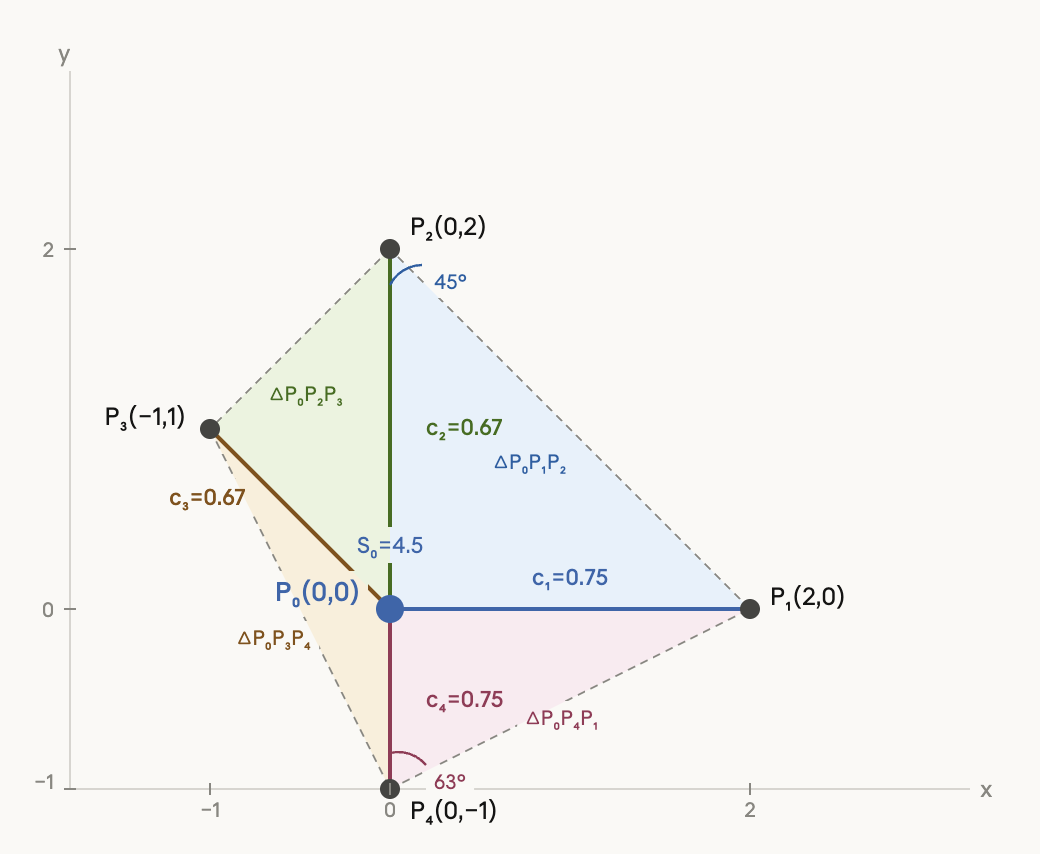
\includegraphics[width=0.75\textwidth]{image/triangle.png}
    \captionof{figure}{三角形网格差分示例：$P_0$ 周围的四个三角单元及权系数 $c_i$}
\end{center}
\end{center}
\begin{dxtips}
 $P_0P_1$ 对应的两个对角分别为 $\angle P_0P_2P_1$ 和 $\angle P_0P_4P_1$。
\end{dxtips}
\begin{example}[三角形网格差分：数值计算]
取内部节点 $P_0=(0,0)$，周围四个邻居节点逆时针排列：
\[
P_1=(2,0),\quad P_2=(0,2),\quad P_3=(-1,1),\quad P_4=(0,-1),
\]
形成四个三角单元 $\triangle P_0P_1P_2$，$\triangle P_0P_2P_3$，$\triangle P_0P_3P_4$，$\triangle P_0P_4P_1$。

\textbf{第一步：对每条边算权系数}

$$c_i = \frac{\cot\theta_i^- + \cot\theta_i^+}{2}$$

其中 $\theta_i^\pm$ 为边 $P_0P_i$ 在相邻两个三角单元中的对角。逐边计算：

\begin{itemize}
  \item 边 $P_0P_1$： $c_1  = 0.75$ ；
 边 $P_0P_2$：$c_2 = 0.67$；
边 $P_0P_3$： $c_3 =  0.67$；
  边 $P_0P_4$：$c_4 =  0.75$
\end{itemize}

所有 $c_i > 0$，内角均不超过 $90°$，离散极值原理成立。

\textbf{第二步：算总面积 $S_0$}

用叉积公式 $S = \frac{1}{2}|\vec{a}\times\vec{b}|$ 逐一计算：
\[
S_{\triangle P_0P_1P_2}=2,\quad
S_{\triangle P_0P_2P_3}=1,\quad
S_{\triangle P_0P_3P_4}=0.5,\quad
S_{\triangle P_0P_4P_1}=1,
\]
故 $S_0 = 4.5$。

\textbf{第三步：写出差分格式}

代入 cotangent formula：
\[
\Delta u\big|_{P_0}
\approx \frac{1}{S_0}\sum_{i=1}^{4}c_i(u_i-u_0)
= \frac{1}{4.5}\bigl[0.75(u_1-u_0)+0.67(u_2-u_0)
+0.67(u_3-u_0)+0.75(u_4-u_0)\bigr],
\]
整理得
\[
\Delta u\big|_{P_0}
\approx \frac{1}{4.5}\bigl[0.75\,u_1+0.67\,u_2+0.67\,u_3+0.75\,u_4-2.84\,u_0\bigr].
\]
即 $u_0$ 处的拉普拉斯值等于邻居的加权平均减去自身，权重 $c_i$ 正比于对角的余切之和。
\end{example}
\begin{note}
    一句话：格林公式把难以在不规则网格上处理的二阶算子，降阶成可以逐段近似的一阶法向导数。
\end{note}
\begin{theorem}[散度定理的统一性]
散度定理（Gauss-Green 定理）
\[
\iint_{\Omega} \nabla \cdot \mathbf{F} \, dA = \oint_{\partial\Omega} \mathbf{F} \cdot \mathbf{n} \, ds
\]
是以下经典结论的共同本质：
\begin{enumerate}
  \item 令 $\mathbf{F} = \nabla u$，则 $\nabla \cdot \mathbf{F} = \Delta u$，即得\textbf{格林公式}
  \[
  \iint_{\Omega} \Delta u \, dA = \oint_{\partial\Omega} \frac{\partial u}{\partial \mathbf{n}} \, ds;
  \]
  \item 令 $\mathbf{F} = \mathbf{E}$，则 $\nabla \cdot \mathbf{E} = \rho/\varepsilon_0$，即得\textbf{高斯定理}
  \[
  \oint_{\partial\Omega} \mathbf{E} \cdot \mathbf{n} \, ds = \frac{Q}{\varepsilon_0};
  \]
  \item 复变函数中的\textbf{柯西积分公式}本质上也是二维散度定理在全纯函数上的体现。
\end{enumerate}
\end{theorem}
\begin{dxtips}
   核心思想就是求点 $P_0$ 的值不好求，用拉普拉斯算子也就是 $\Delta u$，通过点周围一圈的信息来求取。有角度那向就是对发向量求导
\end{dxtips}
\begin{note}[从格林公式到差分格式]
对 $P_0$ 周围的多边形区域 $\Omega_0$ 用格林公式：
\[
\iint_{\Omega_0} \Delta u \, dA = \oint_{\partial \Omega_0} \frac{\partial u}{\partial \mathbf{n}} \, ds.
\]
\textbf{左边：}假设 $\Delta u$ 在 $\Omega_0$ 内近似为常数，提出得
\[
\iint_{\Omega_0} \Delta u \, dA \approx \Delta u\big|_{P_0} \cdot S_0.
\]
\textbf{右边：}$\partial\Omega_0$ 由各三角单元的对边拼成。对每段对边，以对边 $P_iP_{i+1}$ 为例，法向导数近似为
\[
\frac{\partial u}{\partial \mathbf{n}} \approx \frac{u_0 - \bar{u}}{d},
\]
其中 $\bar{u}$ 为对边上的插值，$d$ 为 $P_0$ 到对边的距离。经几何化简，第 $i$ 段对边的贡献为
\[
\frac{\cot\theta_i^- + \cot\theta_i^+}{2}(u_i - u_0),
\]
所有段求和得
\[
\oint_{\partial \Omega_0} \frac{\partial u}{\partial \mathbf{n}} \, ds \approx \sum_{i=1}^{m} c_i(u_i - u_0), \qquad c_i = \frac{\cot\theta_i^- + \cot\theta_i^+}{2}.
\]
\textbf{合并两边}后除以 $S_0$：
\[
\boxed{\Delta u\big|_{P_0} \approx \frac{1}{S_0}\sum_{i=1}^{m} c_i(u_i - u_0).}
\]
格林公式将 $P_0$ 处的二阶算子转化为边界上的一阶法向导数，余切系数 $c_i$ 来自几何化简中的面积与距离关系。
\end{note}